% Generated by capacity_theory; known probability laws, not room measurements.
\begin{figure}[htbp]
\centering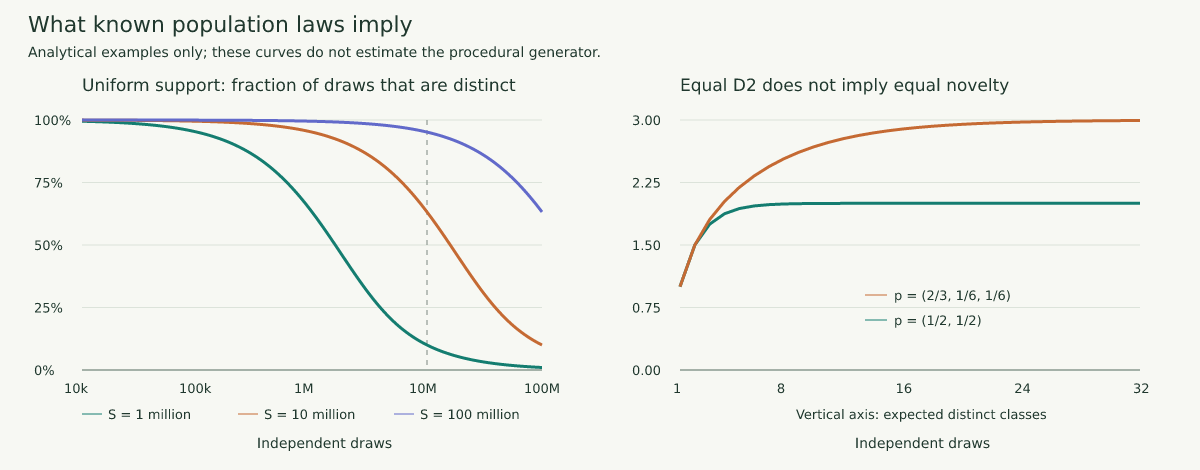
\includegraphics[width=\linewidth]{generated/capacity_scaling.png}
\caption{Analytical occupancy examples, not measured Zeroverse capacity.
Left: distinct fraction for uniform populations with known support; dashed line
marks ten million draws. Right: two populations have the same collision diversity
$D_2=2$ but different occupancy curves and limiting support. A single effective
number does not determine long-run novelty.}
\label{fig:capacity-scaling}
\end{figure}
\begin{table}[htbp]\centering\small
\begin{tabular}{lrrr}\toprule
Known uniform support & Expected distinct & Distinct/draws & Next-draw novelty\\
\midrule
1 million & 1.000 million & 10.00\% & 0.00\% \\
10 million & 6.321 million & 63.21\% & 36.79\% \\
100 million & 9.516 million & 95.16\% & 90.48\% \\
\bottomrule\end{tabular}
\caption{Exact uniform-occupancy formulas at $n=10^7$, rounded for display.
No row estimates the support of this generator.}\label{tab:capacity-oracles}
\end{table}
